\section{Cartesian Coordinates}

\blue{Insert the same content here as from the TAM212 Reference Pages (Positions and Coordinates - Cartesian Coordinates)}

\subsection{Vector Bases}

\blue{Insert the same content here as from the TAM212 Reference Pages (Vectors and Bases - Vector Bases)}

\subsection{Right Hand Rule}

The Cartesian system is a "right-handed" coordinate system, which means that we can use the right-hand rule to determine the direction of the $x, y$ and $z$ axes. In 3D the $x, y, z$ axes are oriented in right-handed order, so that fingers curling from $x$ to $y$ means the thumb points in the $z$ direction.

\begin{figure*}[!h]
\centering
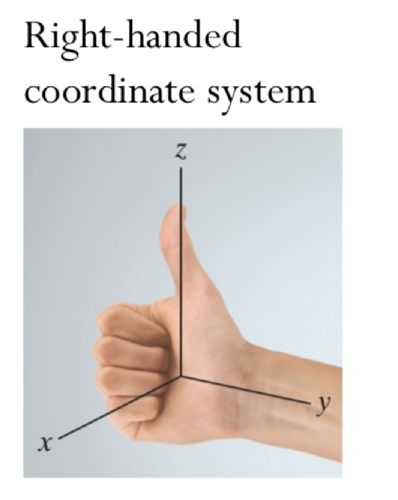
\includegraphics[angle=0, width=2in]{CartCoordFigures/RightHandRule.png}
\vspace{-2mm}
\caption{\small \blue{Taken from TAM 210 Lecture 3 - Slide 3}}
\vspace{-3mm}
\label{Fig:NewtonsLaws}
\end{figure*}


